\chapter{Values and Variables}

\textsc{Perspective}: No feature of the Icon programming language has
a greater impact on the implementation than untyped
variables --- variables that have no specific type associated with
them. This feature originated in Icon's predecessors as a result of a
desire for simplicity and flexibility.

The absence of type declarations reduces the amount that a programmer
has to learn and remember. It also makes programs shorter and
(perhaps) easier to write. The flexibility comes mainly from the
support for heterogeneous aggregates. A list, for example, can contain
a mixture of strings, integers, records, and other lists. There are
numerous examples of Icon programs in which this flexibility leads to
programming styles that are concise and simple. Similarly,
{\textquotedbl}generic{\textquotedbl} procedures, whose arguments can
be of any type, often are useful, especially for modeling experimental
language features.

While these facilities can be provided in other ways, such as by C's
union construct, Icon provides them by the \textit{absence} of
features, which fits with the philosophy of making it easy to write
good programs rather than hard to write bad ones.

The other side of the coin is that the lack of type declarations for
variables makes it impossible for the translator to detect most type
errors and defers type checking until the program is executed. Thus, a
check that can be done only once at translation time in a language
with a strong compile-time type system must be done repeatedly during
program execution in Icon. Furthermore, just as the Icon translator
cannot detect most type errors, a person who is writing or reading an
Icon program does not have type declarations to help clarify the
intent of the program.

Icon also converts arguments to the expected type where possible. This
feature is, nevertheless, separable from type checking; Icon could
have the latter without the former. However, type checking and
conversion are naturally intertwined in the implementation.

As far as the implementation is concerned, untyped variables simplify
the translator and complicate the run-time system.  There is little
the translator can do about types. Many operations are polymorphic,
taking arguments of different types and sometimes performing
significantly different computations, depending on those types. Many
types are convertible to others. Since procedures are data values and
may change meaning during program execution, there is nothing the
translator can know about them. For this reason, the translator does
not attempt any type checking or generate any code for type checking
or conversion. All such code resides in the run-time routines for the
functions and operations themselves.

There is a more subtle way in which untyped variables influence the
implementation. Since any variable can have any type of value at any
time, and can have different types of values at different times, all
values must be the same size.  Furthermore, Icon's rich repertoire of
data types includes values of arbitrary size-lists, tables,
procedures, and so on.

The solution to this problem is the concept of a \textit{descriptor},
which either contains the data for the value, if it is small enough,
or else contains a pointer to the data if it is too large to fit into
a descriptor. The trick, then, is to design descriptors for all of
Icon's data types, balancing considerations of size, ease of type
testing, and efficiency of accessing the actual data.


\section[4.1 Descriptors]{4.1 Descriptors}

Since every Icon value is represented by a descriptor, it is important
that descriptors be as small as possible. On the other hand, a
descriptor must contain enough information to determine the type of
the value that it represents and to locate the actual data. Although
values of some types cannot possibly fit into any fixed-size space, it
is desirable for frequently used, fixed-sized values, such as
integers, to be stored in their descriptors. This allows values of
these types to be accessed directly and avoids the need to provide
storage elsewhere for such values.

If Icon were designed to run on only one kind of computer, the size
and layout of the descriptor could be tailored to the architecture of
the computer. Since the implementation is designed to run on a wide
range of computer architectures, Icon takes an approach similar to
that of C. Its descriptor is composed of ``words,'' which are closely
related to the concept of a word on the computer on which Icon is
implemented. One word is not large enough for a descriptor that must
contain both type information and an integer or a pointer. Therefore,
a descriptor consists of two words, which are designated as the
\textit{d-word} and the \textit{v-word}, indicating that the former
contains descriptive information, while the latter contains the value

%--%\ \ \ \  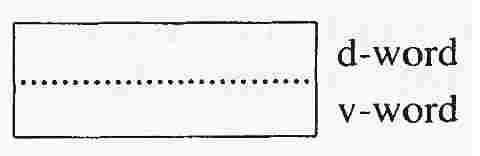
\includegraphics[width=1.602in,height=0.5201in]{ib-img/ib-img005.jpg} 
\begin{picture}(300,50)
\put(100,10){\dvbox{}{}{}}
\put(100,10){\rightboxlabels{d-word}{v-word}}
\end{picture}

The dotted line between the two words of a descriptor is provided for
readability. A descriptor is merely two words, and the fact that these
two words constitute a descriptor is a matter of context.

The v-word of a descriptor may contain either a value, such as an
integer, or a pointer to other data. In C terms. the v-word may
contain a variety of types, including both ints and pointers. On many
computers, C ints and C pointers are the same size. For some
computers, however, C compilers have a memory-model in which integers
are smaller than pointers, which must allow access to a large amount
of memory. In this situation, the C \texttt{long} or \texttt{long
long} type are the same size as C pointers. There are computers with
many different word sizes, but the main considerations in the
implementation of Icon are the accommodation of computers with 32- and
64-bit words and the large-memory model, in which pointers are larger
than integers. In the large-memory model, a v-word must accommodate
the largest of the types.

The d-words of descriptors contain a type code (a small integer) in
their least significant bits and flags in their most significant
bits. There are twelve type codes that correspond to source-language
data types:

\begin{tabular}{l@{\hspace{1in}}l}
\textit{data type} & \textit{type code} \\
null & \texttt{null}\\
integer & \texttt{integer} or \texttt{long}\\
real number & \texttt{real}\\
cset & \texttt{cset}\\
file & \texttt{file}\\
procedure & \texttt{proc}\\
list & \texttt{list}\\
set & \texttt{set}\\
table & \texttt{table}\\
record & \texttt{record}\\
co-expression & \texttt{coexpr}\\
\end{tabular}

Other type codes exist for internal objects, which are on a par with
source-language objects, from an implementation viewpoint, but which
are not visible at the source-language level. The actual values of
these codes are not important, and they are indicated in diagrams by
their type code names.

\subsection[4.1.1. Strings]{4.1.1. Strings}

There is no type code for strings. They have a special representation
in which the d-word contains the length of the string (the number of
characters in it) and the v-word points to the first character in the
string:



\begin{center}
%--%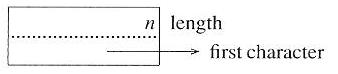
\includegraphics[width=2.4898in,height=0.5193in]{ib-img/ib-img006.jpg}
\begin{picture}(200,32)
\put(0,0){\dvptrbox{\textit{n}}{}{50}{first character}}
\put(0,0){\trboxlabel{length}}
\end{picture}
\end{center}

String descriptors are called \textit{qualifiers}. In order to make
qualifiers more intelligible in the diagrams that follow, a pointer to
a string is followed by the string in quotation marks rather than by
an address. For example, the qualifier for
\texttt{{\textquotedbl}hello{\textquotedbl}} is depicted as

\begin{center}
%--%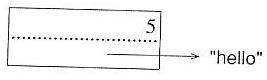
\includegraphics[width=1.9693in,height=0.5598in]{ib-img/ib-img007.jpg}
\begin{picture}(200,32)
\put(0,0){\dvptrbox{5}{}{50}{"hello"}}
\put(0,0){\trboxlabel{length}}
\end{picture}
\end{center}

In order to distinguish qualifiers from other descriptors with type
codes that might be the same as a string length, all descriptors that
are not qualifiers have an n flag in the most significant bit of the
d-word. The d-words of qualifiers do not have this n flag, and string
lengths are restricted to prevent their overflow into this flag
position, the most significant bit of a 32- or 64-bit dword.

\subsection[4.1.2 The Null Value]{4.1.2 The Null Value}

A descriptor for the null value has the form

\begin{center}
%--%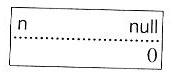
\includegraphics[width=1.5193in,height=0.6598in]{ib-img/ib-img008.jpg}
\begin{picture}(200,32)
\put(0,0){\dvbox{null}{n}{0}}
\end{picture}
\end{center}

As explained previously, the n flag occurs in this and all other
descriptors that are not qualifiers so that strings can be easily and
unambiguously distinguished from all other kinds of values. The value
in the v-word could be any constant value, but zero is useful and
easily identified---and suggests
{\textquotedbl}null.{\textquotedbl}

In the diagrams that follow, a null block-pointer is represented as
\begin{center}
\begin{picture}(200,16)
\put(0,0){\nullptrbox{}}
\end{picture}
\end{center}

\noindent
Icon version 6 used descriptors in blocks to refer to other blocks (see section
4.2). Subsequent versions switched to using pointers.

\subsection[4.1.3 Integers]{4.1.3 Integers}

Icon supports word-size integers at least 32-bits in size. Such
integers therefore are typically C longs, depending on the computer
architecture. As long as it fits, the value of an Icon integer is
stored in the v-word of its descriptor.  For example, the integer
13570 is represented by

\begin{center}
%--%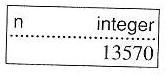
\includegraphics[width=1.2799in,height=0.5492in]{ib-img/ib-img009.jpg}
\begin{picture}(200,32)
\put(0,0){\dvbox{integer}{n}{13750}}
\end{picture}
\end{center}

Note that the \texttt{n} flag distinguishes this descriptor from a string whose
first character might be at the address 13570 and whose length might
have the same value as the type code for integer.

An Icon integer that fits in the v-word is stored there. An integer
that is too large to fit into a word is stored in a data structure
that is pointed to by the v-word, as illustrated in the next
section. The two representations of integers are distinguished by
different internal type codes: integer for integers that are contained
in the v-words of their descriptors and lrgint for integers that are
contained in blocks pointed to by the v-words of their descriptors.
Thus, there are two internal types for one source-language data type.


\section[4.2 Blocks]{4.2 Blocks}

All other types of Icon data are represented by descriptors with
v-words that point to blocks of words. These blocks have a
comparatively uniform structure that is designed to facilitate their
processing during garbage collection.

The first word of every block, called its \textit{title}, contains a
type code. This type code is the same code that is in the type-code
portion of the d-word of a descriptor that points to the block. Some
blocks are fixed in size for all values of a given type. For example,
on a computer with 32-bit words, the source language integer 5,000,000,000 is
stored in a large integer block:

%--%\ \  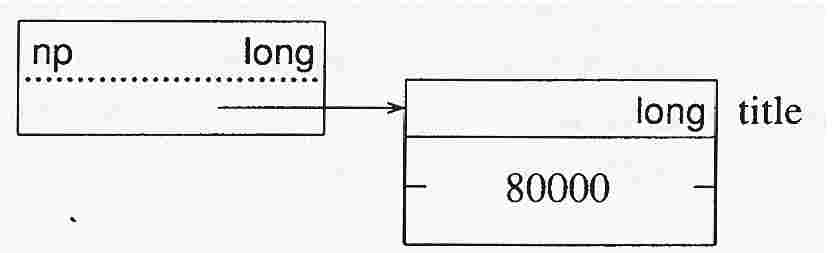
\includegraphics[width=2.778in,height=0.8437in]{ib-img/ib-img010.jpg} 
\begin{picture}(300,80)
\put(0,32){\dvptrbox{lrgint}{np}{60}{}}
\put(140,0){\blklrgbox{lrgint}{5,000,000,000}}
\put(140,17){\trboxlabel{title}}
\end{picture}

\noindent The \texttt{p} flag in the descriptor indicates that the v-word
contains a pointer to a block.

Blocks of some other types, such as record blocks, vary in size from
value to value, but any one block is fixed in size and never grows or
shrinks. If the type code in the title does not determine the size of
the block, the second word in the block contains its size in bytes. In
the diagrams that follow, the sizes of blocks are given for computers
with 32-bit words. The diagrams would be slightly different for
computers with 16-bit words.

Records, which differ in size depending on how many fields they have,
are examples of blocks that contain their sizes.  For example, given
the record declaration

%-% {\ttfamily\mdseries
%-% \ \ \ record complex(r, i)}
\iconline{
\>record complex(r, i)
}

\noindent and

%-% {\ttfamily\mdseries
%-% \ \ \ point := complex(1, 3)}
\iconline{
\>point := complex(1, 3)
}

\noindent the value of \texttt{point} is

%--% \begin{center}
%--% 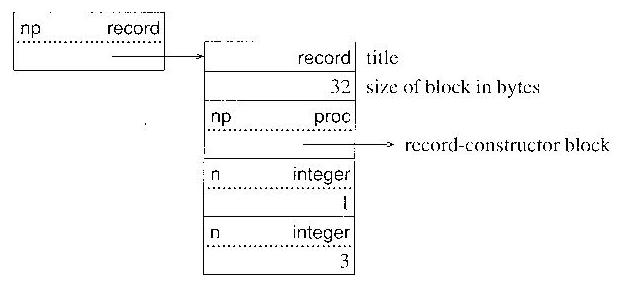
\includegraphics[width=5.3098in,height=2.3193in]{ib-img/ib-img011.jpg}
%--% \end{center}
\begin{picture}(300,150)(-20,0)
\put(0,112){\dvptrbox{record}{np}{60}{}}
\put(140,96){\blkbox{record}{32}}
\put(140,96){\rightboxlabels{title}{size of block in bytes}}
\put(140,80){\wordbox{\textit{id}}}
\put(140,64){\wordptr{50}{record constructor}}
\put(140,32){\dvbox{integer}{n}{1}}
\put(140,0){\dvbox{integer}{n}{3}}
\end{picture}

The record-constructor block contains information that is needed to
resolve field references.

The \textit{id} field is present in many blocks. Its purpose is to
distinguish between different blocks of the same type (for example, it
is used in the computation of the hash value that determines where to
place a value in a table --- see section 7.3 for details). The
\textit{id} field is also printed out by diagnostic routines; it is
incremented for each block created. The runtime system maintains
separate {\em id} counters for blocks of different types.

With the declaration

\iconline{
\>record term(value, code, count)
}

\noindent and

\iconline{
\>word := term("chair", "noun", 4)
}

\noindent the value of word is:

%--% 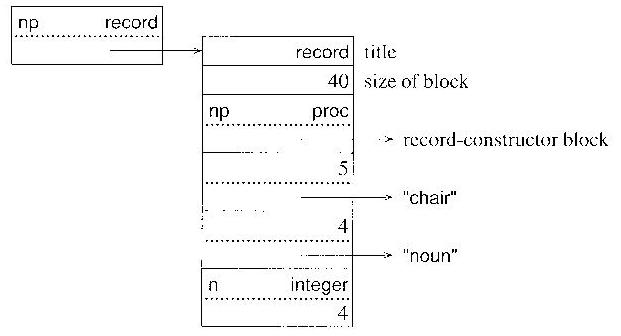
\includegraphics[width=4.6398in,height=2.3799in]{ib-img/ib-img012.jpg}
\begin{picture}(300,190)(-20,0)
\put(0,144){\dvptrbox{record}{np}{60}{}}
\put(140,128){\blkbox{record}{40}}
\put(140,128){\rightboxlabels{title}{size of block}}
\put(140,112){\wordbox{\textit{id}}}
\put(140,96){\wordptr{50}{record-constructor}}
\put(140,64){\dvptrbox{5}{}{50}{"chair"}}
\put(140,32){\dvptrbox{4}{}{50}{"noun"}}
\put(140,0){\dvbox{integer}{n}{4}}
\end{picture}

As illustrated by these examples, blocks may contain descriptors as
well as non-descriptor data. Non-descriptor data comes first in the
block, followed by any descriptors, as illustrated by the preceding
figure. The location of the first descriptor in a block is constant
for all blocks of a given type, which facilitates garbage collection.
Block-pointers may be placed anywhere before the descriptors, but the
garbage collector expects them to be contiguous and in a fixed place
for all blocks of a given type.

Blocks for the remaining types are described in subsequent chapters.

\section[4.3 Variables]{4.3 Variables}

Variables are represented by descriptors, just as values are. This
representation allows values and variables to be treated uniformly in
terms of storage and access. Variables for identifiers point to
descriptors for the corresponding values. Variables always point to
descriptors for values, never to other variables. For example, if

\iconline{
\>  s := "hello"
}

\noindent then a variable for \texttt{s} has the form

%--% 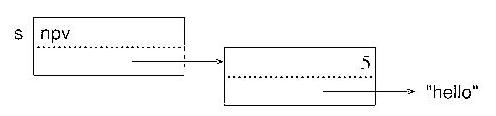
\includegraphics[width=3.8193in,height=0.8492in]{ib-img/ib-img013.jpg}
\begin{picture}(300,64)(-30,0)
\put(0,16){\tlboxlabel{\texttt{s}}}
\put(0,16){\dvptrbox{}{npv}{60}{}}
\put(140,0){\dvptrbox{5}{}{50}{"hello"}}
\end{picture}

\noindent
The v flag distinguishes descriptors for variables from descriptors for values.

The values of local identifiers are kept on a stack, while the values
of global and static identifiers are located at fixed places in
memory. Variables that point to the values of identifiers are created
by icode instructions that correspond to the use of the identifiers in
the program.

Some variables, such as record field references, are computed. A
variable that references a value in a data structure points to the
start of the data structure. The least-significant bits of the d-word
for such a variable contain the offset, in \textit{words}, of the
value descriptor from the top of the block in which the value is
contained. The use of words, rather than bytes, allows larger offsets,
which is important for computers with 16-bit words. For example, the
variable \texttt{word.count} for the record given in the preceding section is

%--% \begin{center}
%--% 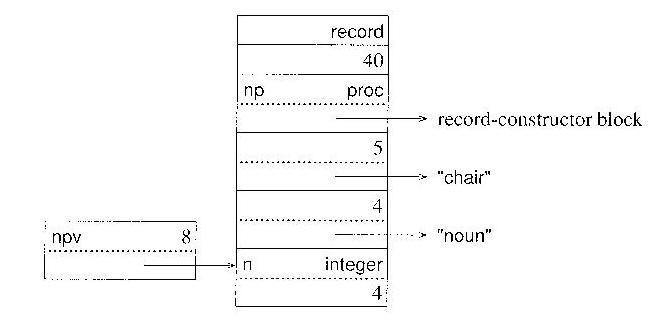
\includegraphics[width=5.2492in,height=2.4098in]{ib-img/ib-img014.jpg}
%--% \end{center}
\begin{picture}(300,180)(-20,0)
\put(0,16){\dvptrbox{8}{npv}{40}{}}
\put(150,128){\blkbox{record}{40}}
\put(120,24){\line(0,1){128}}
\multiput(120,24)(4,0){9}{\line(1,0){2}}
\put(146,24){\vector(1,0){4}}
\put(120,152){\vector(1,0){30}}
\put(150,112){\wordbox{\textit{id}}}
\put(150,96){\wordptr{50}{record-constructor block}}
\put(150,64){\dvptrbox{5}{}{50}{"chair"}}
\put(150,32){\dvptrbox{4}{}{50}{"noun"}}
\put(150,0){\dvbox{integer}{n}{4}}
\end{picture}

Note that the variable \texttt{word.count} cannot be determined at
translation time, since the type of word is not known then and
different record types could have count fields in different positions.

\subsection[4.3.1 Operations on Variables]{4.3.1 Operations on Variables}

There are two fundamentally different contexts in which a variable can
be used: \textit{dereferencing} and \textit{assignment}.

Suppose, as shown previously, that the value of the identifier s is
the string {\textquotedbl}hello{\textquotedbl}. Then a variable
descriptor that points to the value of s and the corresponding value
descriptor for {\textquotedbl}hello{\textquotedbl} have the following
relationship:

In an expression such as \texttt{write(s)}, \texttt{s} is dereferenced
by fetching the descriptor pointed to by the v-word of the variable.

\begin{picture}(300,64)(-30,0)
\put(0,16){\tlboxlabel{\texttt{s}}}
\put(0,16){\dvptrbox{}{npv}{60}{}}
\put(140,0){\dvptrbox{5}{}{50}{"hello"}}
\end{picture}

In the case of assignment, as in

%-% {\ttfamily\mdseries
%-% \ \ \ s := 13570}
\iconline{
\>s := 13570
}

\noindent the value descriptor pointed to by the v-word of the
variable descriptor changed:

%--%\ \  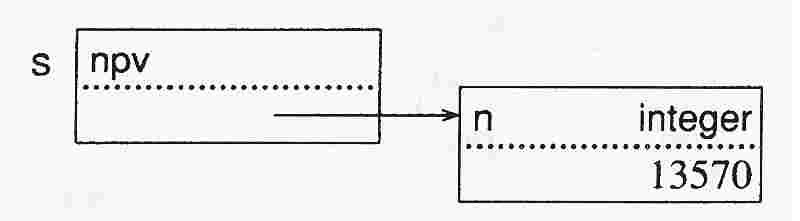
\includegraphics[width=2.6717in,height=0.7374in]{ib-img/ib-img016.jpg} 
\begin{picture}(300,64)(-30,0)
\put(0,16){\tlboxlabel{\texttt{s}}}
\put(0,16){\dvptrbox{}{npv}{60}{}}
\put(140,0){\dvbox{integer}{n}{13570}}
\end{picture}

These operations on variables correspond to indirect load and store
instructions of a typical computer.

\subsection[4.3.2 Trapped Variables]{4.3.2 Trapped Variables}

Icon has several variables with special properties that complicate
assignment and dereferencing. Consider, for example, the keyword
\texttt{\&trace}. Its value must always be an integer. Consequently,
in an assignment such as

%-% {\ttfamily\mdseries
%-% \ \ \ \&trace := \textit{expr}}
\iconline{
\>\&trace := \textit{expr}
}

\noindent the value produced by \textit{expr} must be checked to be
sure that it is an integer. If it is not, an attempt is made to
convert it to an integer, so that in

%-% {\ttfamily\mdseries
%-% \ \ \ \&trace := {\textquotedbl}1{\textquotedbl}}
\iconline{
\>\&trace := "1"
}

\noindent the value assigned to \texttt{\&trace} is the integer
\texttt{1}, not the string \texttt{{\textquotedbl}1{\textquotedbl}}.

There are four keyword variables that require special processing for
assignment: \texttt{\&trace}, \texttt{\&random}, \texttt{\&subject},
and \texttt{\&pos}. The keyword \texttt{\&random} is treated in
essentially the same way that \texttt{\&trace} is. Assignment to
\texttt{\&subject} requires a string value and has the side effect of
assigning the value \texttt{1} to \texttt{\&pos}. Assignment to
\texttt{\&pos} is even more complicated: not only must the value
assigned be an integer, but if it is not positive, it must also be
converted to the positive equivalent with respect to the length of
\texttt{\&subject}. In any event, if the value in the assignment to
\texttt{\&pos} is not in the range of \texttt{\&subject}, the
assignment fails. Dereferencing these keywords, on the other hand,
requires no special processing.

A naive way to handle assignment to these keywords is to check every
variable during assignment to see whether it is one of the four that
requires special processing. This would place a significant
computational burden on every assignment.  Instead, Icon divides
variables into two classes: \textit{ordinary} and
\textit{trapped}. Ordinary variables point to their values as
illustrated previously and require no special processing. Trapped
variables, so called because their processing is
{\textquotedbl}trapped,{\textquotedbl} are distinguished from ordinary
variables by a t flag. Thus, assignment only has to check a single
flag to separate the majority of variables from those that require
special processing.

A trapped-variable descriptor for a keyword points to a block that
contains the value of the keyword, its string name, and a pointer to a
C function that is called when assignment to the keyword is made. For
example, the trapped variable for \texttt{\&trace} is:

%--%\ \  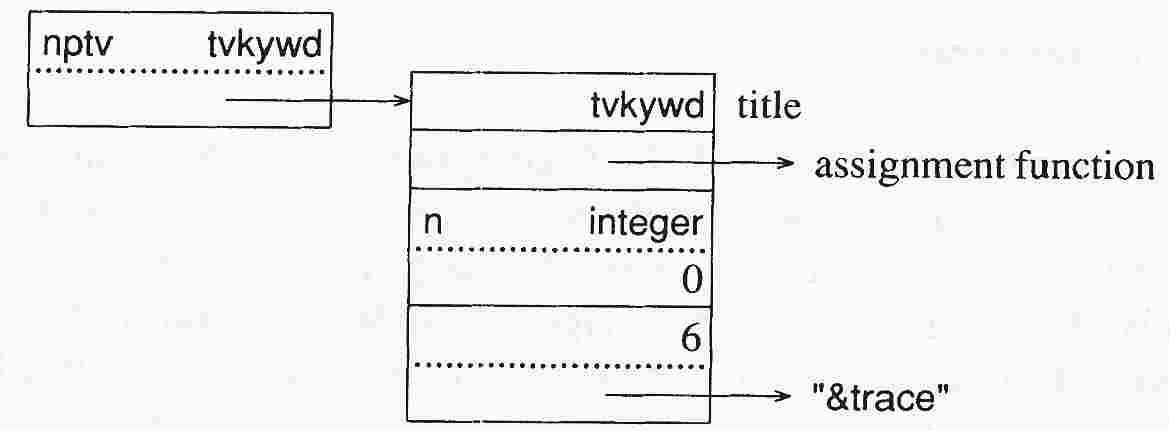
\includegraphics[width=3.9543in,height=1.4398in]{ib-img/ib-img017.jpg} 
\begin{picture}(300,120)(-20,0)
\put(0,80){\dvptrbox{tvkywd}{nptv}{60}{}}
\put(140,64){\blkptrbox{tvkywd}{50}{assignment function}}
\put(140,32){\dvbox{integer}{n}{0}}
\put(140,0){\dvptrbox{6}{}{50}{"\&trace"}}
\end{picture}

It is worth noting that the more conventional approach to handling the
problem of assignment to keywords is to compile special code if a
keyword occurs an assignment context. It is not always possible,
however, to determine the context in which a variable is used in
Icon. Consider a procedure of the form

%-% {\ttfamily\mdseries
%-% \ \ \ procedure diagnose(s)}
%-% 
%-% {\ttfamily\mdseries
%-% \ \ return \&trace}
%-% 
%-% {\ttfamily\mdseries
%-% \ \ \ end}
\iconcode{
\>procedure diagnose(s)\\
\> ...\\
\>return \&trace\\
\>end
}

The semantics of Icon dictate that the result returned in this case
should be a variable, not just its value, so that it is possible to
write an expression such as

%-% {\ttfamily\mdseries
%-% \ \ \ diagnose(s) := 10}
\iconline{
\>diagnose(s) := 10
}

\noindent
which has the effect of assigning the value 10 to \texttt{\&trace}.

The translator has no way of knowing that an assignment to the call
diagnose(s) is equivalent to an assignment to \texttt{\&trace}. In
fact, the translator cannot even determine that the value of diagnose
will be a function when the previous assignment is performed, much
less that it will be the procedure given earlier.

Thus, the trapped-variable mechanism provides a way to handle
uniformly all the situations in which such a keyword can be used.

\section[4.4 Descriptors and Blocks in C]{4.4 Descriptors and Blocks in C}

Descriptors and blocks of data are described and depicted abstractly
in the previous sections of this chapter. In order to understand the
implementation of some aspects of Icon, it is helpful to examine the C
code that actually defines and manipulates data.

The following sections illustrate typical C declarations for the
structures used in the implementation of Icon. Some of the terminology
and operations that appear frequently in the C code are included as
well. Other operations are introduced in subsequent chapters. as they
are needed.

\subsection[4.4.1 Descriptors]{4.4.1 Descriptors}

As mentioned in Sec. 4.1, for C compilers in which ints and pointers
are the same size, the size of a word is the size of an int, while if
pointers are larger than ints, the size of a word is the size of a
long, or a long long. The difference between these models of memory is
handled by typedefs under the control of conditional compilation. Two
constants that characterize the sizes are defined: IntBits and
WordBits. These sizes are used to select appropriate definitions for
signed and unsigned words. The fact that on some 64-bit C compilers a
\texttt{long} is only 32 bits, while on others it is 64 bits,
complicates matters. The symbol \texttt{LongLongWord} indicates this
situation.

\bigskip

% re-insert colors
\iconcode{
\>\#if IntBits != WordBits\\
\>\>{\color{blue}\#ifdef LongLongWord}\\
\>\>\>{\color{blue}typedef long long int word;}\\
\>\>\>{\color{blue}typedef unsigned long long int uword;}\\
\>\>{\color{blue}\#else}\\
\>\>\>typedef long int word;\\
\>\>\>typedef unsigned long uword;\\
\>\>{\color{blue}\#endif}\\
\>\#else \>\>\>\>\>\>\> /* IntBits != WordBits */ \\
\>typedef int word;\\
\>typedef unsigned int uword;\\
\>\#endif
}

A descriptor is declared as a structure:

\iconcode{
\>struct descrip \{\ \ /* descriptor */\\
\>\>word dword;\ \ /*\ \ type field */\\
\>\>union \{\\
\>\>\>word integr;\ \ /*\ \ integer value */\\
% blue
{\color{blue}\#ifdef DescriptorDouble}\\
\>\>\>{\color{blue}double realval;}\\
{\color{blue}\#endif}\\
\>\>\>char *sptr;\ \ /*\ \ pointer to character string */\\
\>\>\>union block *bptr;\ \ /*\ \ pointer to a block */\\
\>\>\>struct descrip *dptr;\ \ /*\ \ pointer to a descriptor */\\
\>\>\} vword;\\
\>\};
}

The v-word of a descriptor is a union that reflects its various uses:
an integer, a pointer to a string, a pointer to a block, or a pointer
to another descriptor (in the case of a variable).

\subsection[4.4.2 Blocks]{4.4.2 Blocks}

Each block type has a structure declaration. For example. the
declaration for record blocks is

\iconcode{
\>struct b\_record \{\>\>\>\>\>\>\>\>\> /* record block */\\
\>\>word title;\>\>\>\>\>\>\>\> /*\ T\_Record */\\
\>\>word blksize;\>\>\>\>\>\>\>\> /*\ \ size of block */\\
\>\> word id;\>\>\>\>\>\>\>\> /*\ \ identification number */\\
\>\>union block *recdesc;\>\>\>\>\>\>\>\> /*   pointer to record constructor */\\
\>\>struct descrip fields[1];\>\>\>\>\>\>\>\> /*\ \ fields */\\
\>\};
}

Blocks for records vary in size, depending on the number of fields
declared for the record type. The size of 1 in

\iconline{
\ \ struct descrip fields[1];
}

\noindent is provided to satisfy the C compiler. Actual blocks for
records are constructed at run time in a region that is managed by
Icon's storage allocator. Such blocks conform to the previous
declaration, but the number of fields varies. The declaration provides
a means of accessing portions of such blocks from C.

The declaration for keyword trapped-variable blocks is

%-% {\ttfamily\mdseries
%-% \ \ \ struct b\_tvkywd \{\ \ \ \ /* keyword trapped variable block */}
%-% 
%-% {\ttfamily\mdseries
%-% \ \ \ \ \ \ word title;\ \ \ \ /*\ \ T Tvkywd */}
%-% 
%-% {\ttfamily\mdseries
%-% \ \ \ \ \ \ int (*putval) ();\ \ /*\ \ assignment function */}
%-% 
%-% {\ttfamily\mdseries
%-% \ \ \ \ \ \ struct descrip kyval;\ \ /*\ \ keyword value */}
%-% 
%-% {\ttfamily\mdseries
%-% \ \ \ \ \ \ struct descrip kyname;/*\ \ keyword name */}
%-% 
%-% {\ttfamily\mdseries
%-% \ \ \ \};}
\iconcode{
\>struct b\_tvkywd \{\ \ \ \ \ \ \ \ /* keyword trapped variable block */\\
\>\>word title;\ \ \ \ \ \ \ \ \ \ \ \ \ /*\ \ T Tvkywd */\\
\>\>int (*putval) ();\ \ \ \ \ \ /*\ \ assignment function */\\
\>\>struct descrip kyval;\ \ \ \ /*\ \ keyword value */\\
\>\>struct descrip kyname;\ \ /*\ \ keyword name */\\
\>\};
}

Note that the title fields of \texttt{b\_record} and
\texttt{b\_tvkywd} contain type codes, as indicated in previous
diagrams. The second field of \texttt{b\_record} is a size as
mentioned previously, but \texttt{b\_tvkywd} has no size field, since
all keyword trapped-variable blocks are the same size, which therefore
can be determined from their type.

The block union given in the declaration of \texttt{struct descrip}
consists of a union of all block types:

%-% {\ttfamily\mdseries
%-% \ \ \ union block \{}
%-% 
%-% {\ttfamily\mdseries
%-% \ \ \ \ \ \ struct b\_real realblk;\newline
%-%  \ \ \ \ \ struct b\_cset cset;\newline
%-%  \ \ \ \ \ struct b\_file file;}
%-% 
%-% {\ttfamily\mdseries
%-% \ \ \ \ \ \ struct b\_proc proc;\newline
%-%  \ \ \ \ \ struct b\_list list;}
%-% 
%-% {\ttfamily\mdseries
%-% \ \ \ \ \ \ struct b\_lelem lelem;\newline
%-%  \ \ \ \ \ struct b\_table table;\newline
%-%  \ \ \ \ \ struct b\_telem telem;\newline
%-%  \ \ \ \ \ struct b\_set set;}
%-% 
%-% 
%-% \ \ \ \ \ \ struct b\_selem selem;\newline
%-%  \ \ \ \ \ struct b\_record record;\newline
%-%  \ \ \ \ \ struct b\_tvsubs tvsubs;\newline
%-%  \ \ \ \ \ struct b\_tvtbl tvtbl;\newline
%-%  \ \ \ \ \ struct b\_refresh refresh;\newline
%-%  \ \ \ \ \ struct b\_coexpr coexpr;\newline
%-%  \ \ \ \ \ struct b\_externl externl;
%-% 
%-% 
%-% \ \ \ \ \ \ struct b\_slots slots;
%-% 
%-% 
%-% \ \ \ \ \ \ struct b\_bignum bignumblk;\newline
%-%  \ \ \ \ \ \};
\iconcode{
\>union block \{\\
\>\>struct b\_real realblk;\\
\>\>struct b\_cset cset;\\
\>\>struct b\_file file;\\
\>\>struct b\_proc proc;\\
\>\>struct b\_list list;\\
\>\>struct b\_lelem lelem;\\
\>\>struct b\_table table;\\
\>\>struct b\_telem telem;\\
\>\>struct b\_set set;\\
\>\>struct b\_selem selem;\\
\>\>struct b\_record record;\\
\>\>struct b\_tvsubs tvsubs;\\
\>\>struct b\_tvtbl tvtbl;\\
\>\>struct b\_refresh refresh;\\
\>\>struct b\_coexpr coexpr;\\
\>\>struct b\_externl externl;\\
\>\>struct b\_slots slots;\\
\>\>struct b\_bignum bignumblk;\\
\>\};
}

Note that there are several kinds of blocks in addition to those that
correspond to source-language data types.

\subsection[4.4.3 Defined Constants]{4.4.3 Defined Constants}

The type codes are defined symbolically:

%-% {\ttfamily\mdseries
%-% \ \ \ \#define T\_Null\ \ \ \ 0}
%-% 
%-% {\ttfamily\mdseries
%-% \ \ \ \#define T\_Integer\ \ \ \ 1}
%-% 
%-% {\ttfamily\mdseries
%-% \ \ \ \#define T\_Lrgint\ \ \ \ 2}
%-% 
%-% {\ttfamily\mdseries
%-% \ \ \ \#define T\_Real\ \ \ \ 3}
%-% 
%-% {\ttfamily\mdseries
%-% \ \ \ \#define T\_Cset\ \ \ \ 4}
%-% 
%-% {\ttfamily\mdseries
%-% \ \ \ \#define T\_File\ \ \ \ 5}
%-% 
%-% {\ttfamily\mdseries
%-% \ \ \ \#define T\_Proc\ \ \ \ 6}
%-% 
%-% {\ttfamily\mdseries
%-% \ \ \ \#define T\_Record\ \ \ \ 7}
%-% 
%-% {\ttfamily\mdseries
%-% \ \ \ \#define T\_List\ \ \ \ 8}
%-% 
%-% {\ttfamily\mdseries
%-% \ \ \ \#define T\_Lelem\ \ \ \ 9}
%-% 
%-% {\ttfamily\mdseries
%-% \ \ \ \#define T\_Set\ \ \ \ 10}
%-% 
%-% {\ttfamily\mdseries
%-% \ \ \ \#define T\_Selem\ \ \ \ 11}
%-% 
%-% {\ttfamily\mdseries
%-% \ \ \ \#define T\_Table\ \ \ \ 12}
%-% 
%-% {\ttfamily\mdseries
%-% \ \ \ \#define T Telem\ \ \ \ 13}
%-% 
%-% {\ttfamily\mdseries
%-% \ \ \ \#define T\_Tvtbl\ \ \ \ 14}
%-% 
%-% {\ttfamily\mdseries
%-% \ \ \ \#define T\_Slots\ \ \ \ 15}
%-% 
%-% {\ttfamily\mdseries
%-% \ \ \ \#define T\_Tvsubs\ \ \ \ 16}
%-% 
%-% {\ttfamily\mdseries
%-% \ \ \ \#define T\_Refresh\ \ \ \ 17}
%-% 
%-% {\ttfamily\mdseries
%-% \ \ \ \#define T\_Coexpr\ \ \ \ 18}
%-% 
%-% {\ttfamily\mdseries
%-% \ \ \ \#define T\_External\ \ \ \ 19}
%-% 
%-% {\ttfamily\mdseries
%-% \ \ \ \#define T\_Kywdint\ \ \ \ 20}
%-% 
%-% {\ttfamily\mdseries
%-% \ \ \ \#define T\_Kywdpos\ \ \ \ 21}
%-% 
%-% {\ttfamily\mdseries
%-% \ \ \ \#define T\_Kywdsubj\ \ \ \ 22}
\iconcode{
\>\#define T\_Null\ \ \ \ 0\\
\>\#define T\_Integer\ \ \ \ 1\\
\>\#define T\_Lrgint\ \ \ \ 2\\
\>\#define T\_Real\ \ \ \ 3\\
\>\#define T\_Cset\ \ \ \ 4\\
\>\#define T\_File\ \ \ \ 5\\
\>\#define T\_Proc\ \ \ \ 6\\
\>\#define T\_Record\ \ \ \ 7\\
\>\#define T\_List\ \ \ \ 8\\
\>\#define T\_Lelem\ \ \ \ 9\\
\>\#define T\_Set\ \ \ \ 10\\
\>\#define T\_Selem\ \ \ \ 11\\
\>\#define T\_Table\ \ \ \ 12\\
\>\#define T Telem\ \ \ \ 13\\
\>\#define T\_Tvtbl\ \ \ \ 14\\
\>\#define T\_Slots\ \ \ \ 15\\
\>\#define T\_Tvsubs\ \ \ \ 16\\
\>\#define T\_Refresh\ \ \ \ 17\\
\>\#define T\_Coexpr\ \ \ \ 18\\
\>\#define T\_External\ \ \ \ 19\\
\>\#define T\_Kywdint\ \ \ \ 20\\
\>\#define T\_Kywdpos\ \ \ \ 21\\
\>\#define T\_Kywdsubj\ \ \ \ 22
}

The type codes in diagrams are abbreviated, as indicated by previous examples.


The defined constants for d-word flags are

%-% {\ttfamily\mdseries
%-% \ \ \ n\ \ \ \ F\_Nqual}
%-% 
%-% {\ttfamily\mdseries
%-% \ \ \ p\ \ \ \ F\_Ptr}
%-% 
%-% {\ttfamily\mdseries
%-% \ \ \ v\ \ \ \ F\_Var}
%-% 
%-% {\ttfamily\mdseries
%-% \ \ \ t\ \ \ \ F\_Tvar}
\iconcode{
\>n\ \ \ \ F\_Nqual\\
\>p\ \ \ \ F\_Ptr\\
\>v\ \ \ \ F\_Var\\
\>t\ \ \ \ F\_Tvar
}

The values of these flags depend on the word size of the computer.


The d-words of descriptors are defined in terms of flags and type codes:

%-% {\ttfamily\mdseries
%-% \ \ \ \#define D\_Null\ \ \ \ (T\_Null {\textbar} F\_Nqual)}
%-% 
%-% {\ttfamily\mdseries
%-% \ \ \ \#define D\_Integer\ \ \ \ (T\_Integer {\textbar} F\_Nqual)}
%-% 
%-% {\ttfamily\mdseries
%-% \ \ \ \#define D\_Long\ \ \ \ (T\_Long {\textbar} F\_Ptr {\textbar} F\_Nqual)}
%-% 
%-% {\ttfamily\mdseries
%-% \ \ \ \#define D\_Real\ \ \ \ (T\_Real {\textbar} F\_Ptr {\textbar} F\_Nqual)}
%-% 
%-% {\ttfamily\mdseries
%-% \ \ \ \#define D\_Cset\ \ \ \ (T\_Cset {\textbar} F\_Ptr {\textbar} F\_Nqual)}
%-% 
%-% {\ttfamily\mdseries
%-% \ \ \ \#define D\_File\ \ \ \ (T\_File {\textbar} F\_Ptr {\textbar} F\_Nqual)}
%-% 
%-% {\ttfamily\mdseries
%-% \ \ \ \#define D\_Proc\ \ \ \ (T\_Proc {\textbar} F\_Ptr {\textbar} F\_Nqual)}
%-% 
%-% {\ttfamily\mdseries
%-% \ \ \ \#define D\_List\ \ \ \ (T\_List {\textbar} F\_Ptr {\textbar} F\_Nqual)}
%-% 
%-% {\ttfamily\mdseries
%-% \ \ \ \#define D\_Table\ \ \ \ (T\_Table {\textbar} F\_Ptr {\textbar} F\_Nqual)}
%-% 
%-% {\ttfamily\mdseries
%-% \ \ \ \#define D\_Set\ \ \ \ (T\_Set {\textbar} F\_Ptr {\textbar} F\_Nqual)}
%-% 
%-% {\ttfamily\mdseries
%-% \ \ \ \#define D\_Selem\ \ \ \ (T\_Selem {\textbar} F\_Ptr {\textbar} F\_Nqual)}
%-% 
%-% {\ttfamily\mdseries
%-% \ \ \ \#define D\_Record\ \ \ \ (T\_Record {\textbar} F\_Ptr {\textbar} F\_Nqual)}
%-% 
%-% {\ttfamily\mdseries
%-% \ \ \ \#define D\_Telem\ \ \ \ (T\_Telem {\textbar} F\_Ptr {\textbar} F\_Nqual)}
%-% 
%-% {\ttfamily\mdseries
%-% \ \ \ \#define D\_Lelem\ \ \ \ (T\_Lelem {\textbar} F\_Ptr {\textbar} F\_Nqual)}
%-% 
%-% {\ttfamily\mdseries
%-% \ \ \ \#define D\_Tvsubs\ \ \ \ (T\_Tvsubs {\textbar} D\_Tvar)}
%-% 
%-% {\ttfamily\mdseries
%-% \ \ \ \#define D\_Tvtbl\ \ \ \ (T Tvtbl {\textbar} D\_Tvar)}
%-% 
%-% {\ttfamily\mdseries
%-% \ \ \ \#define D\_Tvkywd\ \ \ \ (T\_Tvkywd {\textbar} D\_Tvar)}
%-% 
%-% {\ttfamily\mdseries
%-% \ \ \ \#define D\_Coexpr\ \ \ \ (T\_Coexpr {\textbar} F\_Ptr {\textbar} F\_Nqual)}
%-% 
%-% {\ttfamily\mdseries
%-% \ \ \ \#define D\_Refresh\ \ \ \ (T\_Refresh {\textbar} F\_Ptr {\textbar} F\_Nqual)}
%-% 
%-% {\ttfamily\mdseries
%-% \ \ \ \#define D\_Var\ \ \ \ (F\_Var {\textbar} F\ \ \_Nqual {\textbar} F\ \ \_Ptr)}
%-% 
%-% {\ttfamily\mdseries
%-% \ \ \ \#define D\_Tvar\ \ \ \ (D\_Var {\textbar} F\_Tvar)}
\iconcode{
\>\#define D\_Null\ \ \ \ (T\_Null | F\_Nqual)\\
\>\#define D\_Integer\ \ \ \ (T\_Integer | F\_Nqual)\\
\>\#define D\_Lrgint\ \ \ \ (T\_Lrgint | F\_Ptr | F\_Nqual)\\
\>\#define D\_Real\ \ \ \ (T\_Real | F\_Ptr | F\_Nqual)\\
\>\#define D\_Cset\ \ \ \ (T\_Cset | F\_Ptr | F\_Nqual)\\
\>\#define D\_File\ \ \ \ (T\_File | F\_Ptr | F\_Nqual)\\
\>\#define D\_Proc\ \ \ \ (T\_Proc | F\_Ptr | F\_Nqual)\\
\>\#define D\_List\ \ \ \ (T\_List | F\_Ptr | F\_Nqual)\\
\>\#define D\_Table\ \ \ \ (T\_Table | F\_Ptr | F\_Nqual)\\
\>\#define D\_Set\ \ \ \ (T\_Set | F\_Ptr | F\_Nqual)\\
\>\#define D\_Selem\ \ \ \ (T\_Selem | F\_Ptr | F\_Nqual)\\
\>\#define D\_Record\ \ \ \ (T\_Record | F\_Ptr | F\_Nqual)\\
\>\#define D\_Telem\ \ \ \ (T\_Telem | F\_Ptr | F\_Nqual)\\
\>\#define D\_Lelem\ \ \ \ (T\_Lelem | F\_Ptr | F\_Nqual)\\
\>\#define D\_Tvsubs\ \ \ \ (T\_Tvsubs | D\_Tvar)\\
\>\#define D\_Tvtbl\ \ \ \ (T Tvtbl | D\_Tvar)\\
\>\#define D\_Tvkywd\ \ \ \ (T\_Tvkywd | D\_Tvar)\\
\>\#define D\_Coexpr\ \ \ \ (T\_Coexpr | F\_Ptr | F\_Nqual)\\
\>\#define D\_Refresh\ \ \ \ (T\_Refresh | F\_Ptr | F\_Nqual)\\
\>\#define D\_Var\ \ \ \ (F\_Var | F\ \ \_Nqual | F\ \ \_Ptr)\\
\>\#define D\_Tvar\ \ \ \ (D\_Var | F\_Tvar)
}

As indicated previously, flags, type codes, and d-words are
distinguished by the prefixes \texttt{F\_}, \texttt{T\_}, and
\texttt{D\_}, respectively.

\subsection[4.4.4 RTL Coding]{4.4.4 RTL Coding}

Since the optimizing compiler was introduced in versions 8 and 9 of
Icon, the routines for the run-time system use an extended C syntax
called RTL (for Run-Time Language) that encodes the type information
for arguments and results. Some of these are illustrated by the RTL
function for the Icon operator \texttt{*x}, which produces the size of
\texttt{x}:

%-% {\ttfamily\mdseries
%-% \ \ \ operator\{1\} * size(x)}
%-% 
%-% {\ttfamily\mdseries
%-% \ \ \ abstract \{ return integer \}}
%-% 
%-% {\ttfamily\mdseries
%-% \ \ \ type\_case x of \{}
%-% 
%-% {\ttfamily\mdseries
%-% \ \ \ \ \ \ string: inline \{ return C\_integer StrLen(x); \}}
%-% 
%-% {\ttfamily\mdseries
%-% \ \ \ \ \ \ list: inline \{ return C\_integer BlkD(x,List)-{\textgreater}size; \}}
%-% 
%-% {\ttfamily\mdseries
%-% \ \ \ \ \ \ table: inline \{ return C\_integer BlkD(x,Table)-{\textgreater}size; \}}
%-% 
%-% {\ttfamily\mdseries
%-% \ \ \ \ \ \ set: inline \{ return C\_integer BlkD(x,Set)-{\textgreater}size; \}}
%-% 
%-% {\ttfamily\mdseries
%-% \ \ \ \ \ \ cset: inline \{}
%-% 
%-% {\ttfamily\mdseries
%-% \ \ \ \ \ \ \ \ \ register word i = BlkD(x,Cset)-{\textgreater}size;}
%-% 
%-% {\ttfamily\mdseries
%-% \ \ \ \ \ \ \ \ \ if (i {\textless} 0) i = cssize(\&x);}
%-% 
%-% {\ttfamily\mdseries
%-% \ \ \ \ \ \ \ \ \ return C\_integer i;}
%-% 
%-% {\ttfamily\mdseries
%-% \ \ \ \ \ \ \ \ \ \}}
%-% 
%-% {\ttfamily\mdseries
%-% \ \ \ \ \ \ ...}
%-% 
%-% {\ttfamily\mdseries
%-% \ \ \ \ \ \ default: \{}
%-% 
%-% {\ttfamily\mdseries
%-% \ \ \ \ \ \ \ \ \ \ \ \ /*}
%-% 
%-% {\ttfamily\mdseries
%-% \ \ \ \ \ \ \ \ \ \ \ \ \ * Try to convert it to a string.}
%-% 
%-% {\ttfamily\mdseries
%-% \ \ \ \ \ \ \ \ \ \ \ \ \ */}
%-% 
%-% {\ttfamily\mdseries
%-% \ \ \ \ \ \ \ \ \ \ \ if !cnv:tmp\_string(x) then}
%-% 
%-% {\ttfamily\mdseries
%-% \ \ \ \ \ \ \ \ \ \ \ \ \ \ runerr(112, x);\ \ /* no notion of size */}
%-% 
%-% {\ttfamily\mdseries
%-% \ \ \ \ \ \ \ \ \ \ \ inline \{}
%-% 
%-% {\ttfamily\mdseries
%-% \ \ \ \ \ \ \ \ \ \ \ \ \ \ return C\_integer StrLen(x);}
%-% 
%-% {\ttfamily\mdseries
%-% \ \ \ \ \ \ \ \ \ \ \ \ \ \ \}}
%-% 
%-% 
%-% \ \ \ \ \ \ \ \ \ \ \ \}
%-% 
%-% 
%-% \ \ \ \ \ \ \}
%-% 
%-% {\ttfamily
%-% end}
\iconcode{
\>operator\{1\} * size(x)\\
\>abstract \{ return integer \}\\
\>type\_case x of \{\\
\>\>string: inline \{ return C\_integer StrLen(x); \}\\
\>\>list: inline \{ return C\_integer BlkD(x,List)->size; \}\\
\>\>table: inline \{ return C\_integer BlkD(x,Table)->size; \}\\
\>\>set: inline \{ return C\_integer BlkD(x,Set)->size; \}\\
\>\>cset: inline \{\\
\>\>\>register word i = BlkD(x,Cset)->size;\\
\>\>\>if (i < 0) i = cssize(\&x);\\
\>\>\>return C\_integer i;\\
\>\>\>\}\\
\>\>...\\
\>\>default: \{\\
\>\>\>\>/*\\
\>\>\>\>\ * Try to convert it to a string.\\
\>\>\>\>\ */\\
\>\>\>\ \ if !cnv:tmp\_string(x) then\\
\>\>\>\>\ \ runerr(112, x);\ \ /* no notion of size */\\
\>\>\>\ \ inline \{\\
\>\>\>\>\ \ return C\_integer StrLen(x);\\
\>\>\>\>\ \ \}\\
\>\>\>\ \ \}\\
\>\>\}\\
end
}

\texttt{operator} is an RTL construct that performs several
operations. One of these operations is to provide a C function
declaration. Since the function is called by the interpreter, the
header is somewhat different from what it would be if \texttt{size}
were called directly. The details are described in Chapter 8.

The arguments of the Icon operation are referred to via named
descriptors, such as \texttt{x}. The result that is produced is also a
descriptor.

RTL extends C's \texttt{return} statement to include type information,
with which the d-word of the return value is set to
\texttt{D\_lnteger}, since the returned value is a
\texttt{C\_integer}. Next, the \texttt{type\_case} selects different
branches of code depending on the type of x. In the generated code
there is a test to determine if descriptor \texttt{x} holds a
qualifier. \texttt{Qual()} is a macro that is defined as

%-% {\ttfamily\mdseries
%-% \ \ \ \#define Qual(d)\ \ (!((d).dword \& F\_Nqual))}
\iconline{
\>\#define Qual(d)\ \ (!((d).dword \& F\_Nqual))
}

If \texttt{x} is a qualifier, its length is placed in the v-word of
the return value descriptor, using the macros IntVal and StrLen, which
are defined as

%-% {\ttfamily\mdseries
%-% \ \ \ \#define IntVal(d)\ \ ((d).vword.integr)}
%-% 
%-% {\ttfamily\mdseries
%-% \ \ \ \#define StrLen(d)\ \ ((d).dword)}
\iconcode{
\>\#define IntVal(d)\ \ ((d).vword.integr)\\
\>\#define StrLen(d)\ \ ((d).dword)
}

If \texttt{x} is not a qualifier, then the size depends on the
type. The macro \texttt{Type()} isolates the type code

%-% {\ttfamily\mdseries
%-% \ \ \ \#define Type(d)\ \ ((d).dword \& TypeMask)}
\iconline{
\>\#define Type(d)\ \ ((d).dword \& TypeMask)
}

\noindent where the value of \texttt{TypeMask} is 63, providing
considerable room for additions to Icon's internal types.

For most Icon types that are represented by blocks, their
source-language size is contained in their \texttt{size} field. The
macro \texttt{BlkLoc()} accesses a pointer in the v-field of a
descriptor and is defined as

%-% {\ttfamily\mdseries
%-% \ \ \ \#define BlkLoc(d) ((d).vword.bptr)}
\iconline{
\>\#define BlkLoc(d) ((d).vword.bptr)
}

A more specialized macro \texttt{BlkD()} wraps uses of
\texttt{BlkLoc()} and subsequent union member access, allowing
descriptor-block consistency to be verified at run-time if desired.


If the type is not one of those given, the final task is an attempt to
convert \texttt{x} to a string. The RTL expression
\texttt{cnv:tmp\_string()} does this, using local temporary
buffer. The value of \texttt{x} is changed accordingly. A fixed-sized
buffer can be used, since there is a limit to the size of a string
that can be obtained by converting other types. This limit is 256,
which is reached only for conversion of \texttt{\&cset}. The
conversion may fail, as for \texttt{*\&null}, which is signaled by the
return value 0 from \texttt{cnv:tmp\_string()}. In this case, program
execution is terminated with a run-time: error message, using
\texttt{runerr()}. If the conversion is successful, the size is placed
in the v-word of the result, as is the case if \texttt{x} was a
qualifier originally.

\textsc{Retrospective}: Descriptors provide a uniform way of
representing Icon values and variables. Since descriptors for all
types of data are the same size, there are no problems with assigning
different types of values to a variable---they all fit.

The importance of strings is reflected in the separation of
descriptors into two classes---qualifiers and nonqualifiers---by the n
flag. The advantages of the qualifier representation for strings are
discussed in Chapter 5.

It is comparatively easy to add a new type to Icon. A new type code is
needed to distinguish it from other types. If the possible values of
the new type are small enough to fit into the v-word, as is the case
for integers, no other data is needed. For example, the value of a
character data type could be contained in its descriptor. For types
that have values that are too large to fit into a v-word, pointers to
blocks containing the data are placed in the v-words instead. Lists,
sets, and tables are examples of data types that are represented this
way. See Chapters 6 and 7.

\bigskip

\noindent\textbf{EXERCISES}

\noindent\textbf{4.1} Give examples of Icon programs in which
heterogeneous aggregates are used in significant ways.

\noindent\textbf{4.2} Design a system of type declarations for Icon so
that the translator could do type checking. Give special consideration
to aggregates, especially those that may change in size during program
execution. Do this from two perspectives: (a) changing the semantics
of Icon as little as possible, and (b) maximizing ,the type checking
that can be done by the translator at the expense of flexibility in
programming.

\noindent\textbf{4.3} Suppose that functions in Icon were not
first-class values and that their meanings were bound at translation
time. How much could the translator do in the way of error checking?

\noindent\textbf{4.4} Compile a list of all Icon functions and
operators. Are there any that do not require argument type checking?
Are there any that require type checking but not conversion? Identify
those that are polymorphic. For the polymorphic ones, identify the
different kinds of computations that are performed depending on the
types of the arguments.

\noindent\textbf{4.5} Compose a table of all type checks and
conversions that are required for Icon functions and operators.

\noindent\textbf{4.6} To what extent would the implementation of Icon
be simplified if automatic type conversion were not supported? How
would this affect the programmer?

\noindent\textbf{4.7} Why is it desirable for string qualifiers not to have
flags and for all other kinds of descriptors to have flags indicating they
are not qualifiers, rather than the other way around?

\noindent\textbf{4.8} Is the n flag that distinguishes string qualifiers
from all other descriptors really necessary? If not, explain how to
distinguish the different types of descriptors without this flag.

\noindent\textbf{4.9} On computers with extremely limited address
space, two-word descriptors may be impractically large. Describe how
one-word descriptors might be designed, discuss how various types
might be represented, and describe the ramifications for storage
utilization and execution speed.

\noindent\textbf{4.10} Identify the diagrams in this chapter that
would be different if they were drawn for a computer with 16-bit
words.  Indicate the differences.

\noindent\textbf{4.11} There is nothing in the nature of keywords that
requires them to be processed in a special way for assignment but not
for dereferencing. Invent a new keyword that is a variable that
requires processing when it is dereferenced. Show how to generalize
the keyword trapped-variable mechanism to handle such cases.

\noindent\textbf{4.12} List all the syntactically distinct cases in which the
translator can determine whether a keyword variable is used in an
assignment or dereferencing context.

\noindent\textbf{4.13} What would be gained if special code were compiled for
those cases in which the context for keyword variables could be determined?
